\section{Neural Turing Machines}
Neural Turing Machines, 2014 yılında Graves ve arkadaşları tarafından önerilmiştir. Turing makineleri prensibini temel alır ve bir dizi bellek ve kontrol mekanizması kullanarak karmaşık görevleri gerçekleştirmek için tasarlanmıştır. Bellek bandı (Memory Tape) adı verilen bir harici bellek depolama birimine sahiptir. Bu bellek bandı, modelin geçmiş deneyimleri ve bilgilerini depolar. Bellek bandına yazma ve okuma işlemlerini gerçekleştirme için okuma kafalarına sahiptir. Bu kafalar bellek bandına veri yazıp okuyabilir. Bellek bandı ve  başların kontrolünü de bir kontrol mekanizması sağlar.

\begin{figure}[h]
    \centering
    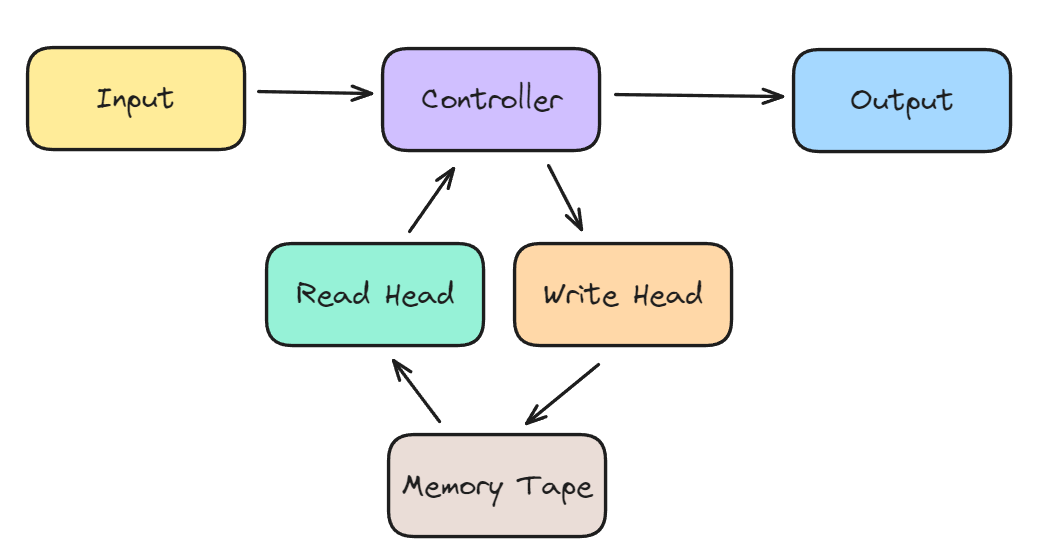
\includegraphics[width=1\textwidth]{images/neural_tuning_machines.png}
    \caption{Sinirsel Turing makinesi mimarisi.}
    \label{fig:enter-label}
\end{figure}

\newpage